\documentclass[11pt]{article}
\usepackage[margin=1in]{geometry}
\usepackage{graphicx,booktabs,amsmath,amssymb,microtype,hyperref,xcolor}
\hypersetup{colorlinks=true,linkcolor=[HTML]{0B1F3A},citecolor=[HTML]{0B1F3A},urlcolor=[HTML]{0B1F3A}}
\title{\textbf{The Gate Was the Wrong Shape}\\[2pt]
\large Measuring a Deployed Triage Engine Against the Formal Specification of Its Own Estate}
\author{Stephen P. Lutar Jr.\\ SZL Holdings}
\date{b077521}
\begin{document}\maketitle

\begin{abstract}
\noindent
We report a deployed, receipt-bearing triage engine that does not yet perform its task, and argue that
the transferable contribution is the measurement discipline rather than the engine. Three results are
established by measurement against artefacts published independently of this work. First, the engine's
aggregator satisfies monotonicity, positive homogeneity, idempotence and boundedness, and violates
permutation invariance on 447 of 895 strictly positive axis vectors, placing
it outside the uniqueness characterisation its own estate proves for the equal-weight geometric mean.
Second, routed against 100 human-labelled rows of the canonical thirteen-axis governance
gate, the engine's compensatory multiplicative rule admits what the non-compensatory conjunctive gate
refuses on 35 rows; errors concentrate on the axes carrying the looser floor, so a
multiplicative aggregator systematically erases a deliberate policy distinction. Third, a leakage gate
transplanted from the estate's own benchmark harness refuses this work's training corpus at a maximum
char-5gram Jaccard of 0.8378, exceeding the value that vetoed a
predecessor adapter after that adapter had passed its behavioural gate on all held-out rows. We record
13 retractions, 9 of them corrections to claims made earlier in this
same work, in an append-only ledger with a test preventing each retracted claim from reappearing. No
model is trained, no baseline is beaten, and no winner is named.
\end{abstract}

\section{Introduction}
A system can be wrong in two ways that look identical from outside: it can compute the right function
badly, or compute the wrong function well. Benchmarks detect the first. The second survives because the
score is real.

This paper is a case study in detecting the second. The engine under study is a deterministic triage
classifier with hash-chained receipts, deployed and passing its own suite. We measure it not against a
leaderboard but against the formal specification published by the organisation that built it: a Lean~4
formalisation of a trust aggregator, a thirteen-axis conjunctive governance gate with human labels, and
a benchmark harness whose leakage check refuses rather than reports. Each comparison was available before
this work began. None had been performed.

\section{The aggregator computes the wrong function well}
The estate defines its trust invariant as the equal-weight geometric mean $\Lambda_k(x)=(\prod_i x_i)^{1/k}$,
with symmetry among its stated properties, and machine-checks that unconditional uniqueness under those
properties is \emph{false} by exhibiting the maximum aggregator as a counterexample. A separate,
kernel-clean result establishes uniqueness among aggregators that additionally factor multiplicatively:
factorisation plus normalisation forces the exponents to sum to one, and symmetry forces them equal.

The deployed engine aggregates four axes with unequal weights. It factors multiplicatively and its
exponents sum to one, and it is therefore excluded from that uniqueness result by exactly one property:
symmetry. Figure~\ref{fig:prop} reports the measurement.

\begin{figure}[t]\centering
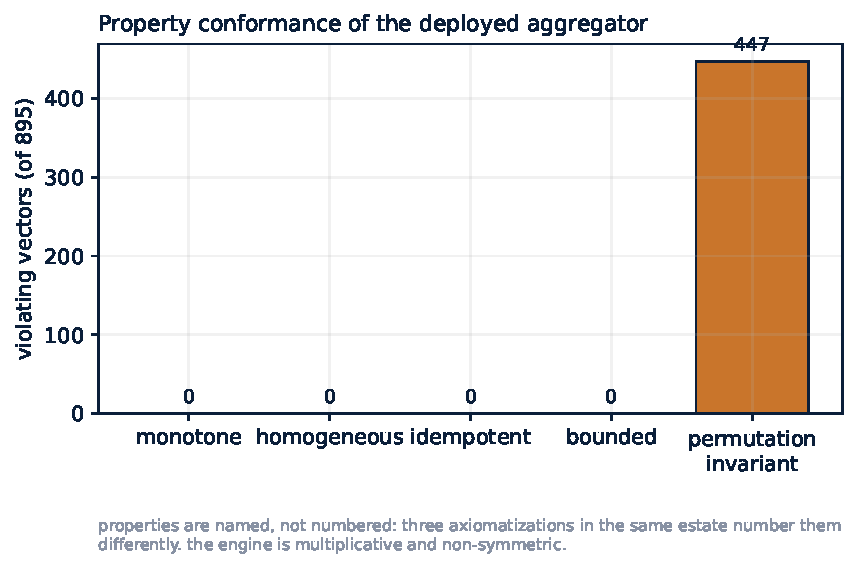
\includegraphics[width=0.78\textwidth]{figures/fig3_property_conformance.pdf}
\caption{Property conformance over 895 strictly positive axis vectors drawn from the live
corpus. Four properties hold exactly; symmetry fails on 447 vectors, which are precisely
those whose components differ.}\label{fig:prop}
\end{figure}

We name properties rather than numbering them. The same estate numbers them three different ways across
three formalisations, so an axiom index is not a stable identifier.

\section{The gate is the wrong shape}
The estate's production governance decision is a thirteen-axis conjunctive gate with a per-axis floor:
every axis must clear its own floor independently. Two axes carry a floor of $0.95$ and the remaining
eleven carry $0.90$. A published split of 100 labelled rows allows direct comparison.

\begin{figure}[t]\centering
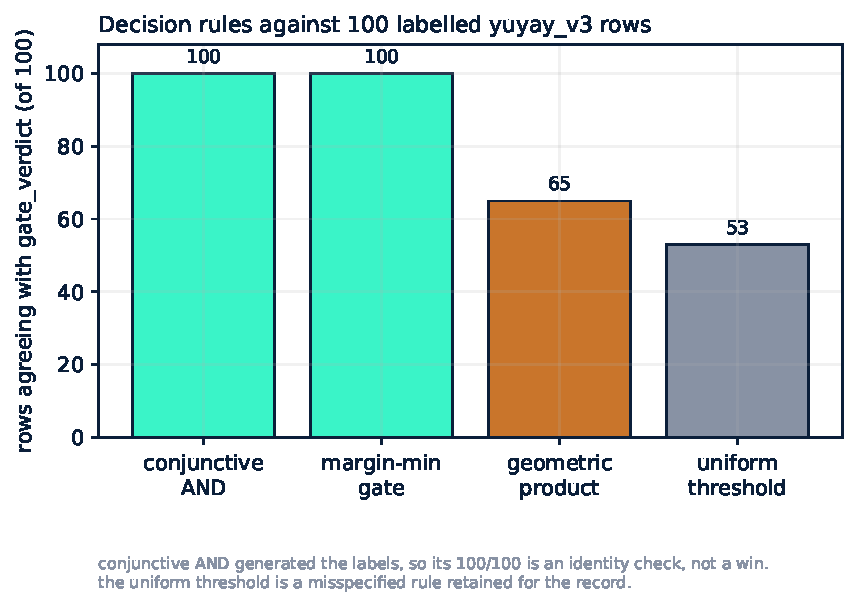
\includegraphics[width=0.78\textwidth]{figures/fig1_decision_rules.pdf}
\caption{Four decision rules against the labelled verdicts. The conjunctive rule generated the labels,
so its perfect agreement is an identity check rather than a result. The margin-min rule
$\min_a(s_a-f_a)\ge 0$ is algebraically identical to the conjunction, which unifies the estate's
deny-by-default uniqueness theorem with its production gate.}\label{fig:rules}
\end{figure}

\begin{figure}[t]\centering
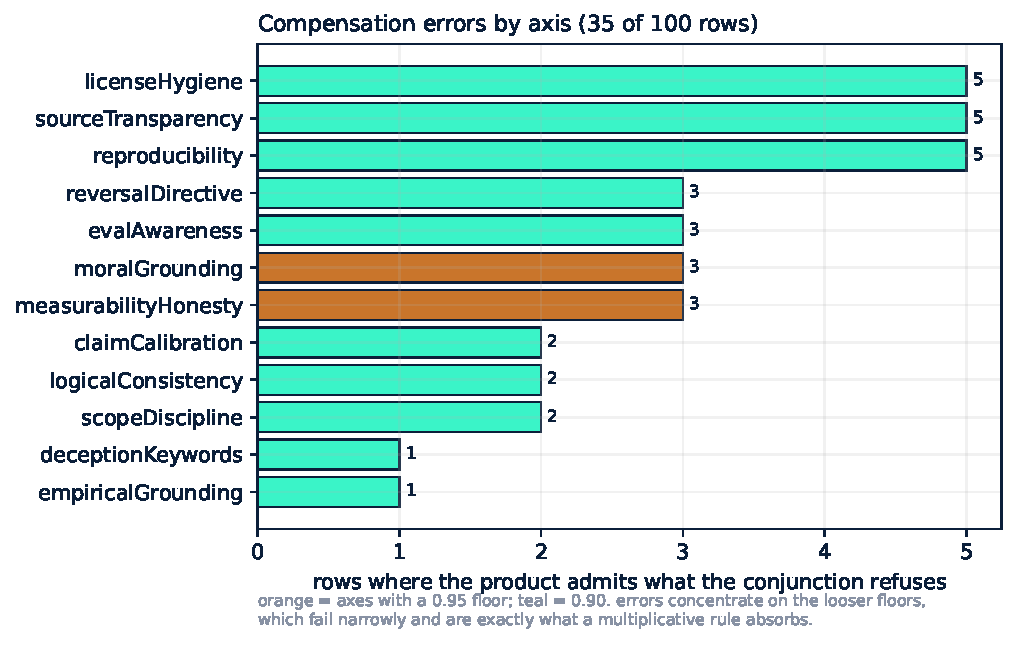
\includegraphics[width=0.74\textwidth]{figures/fig2_compensation_by_axis.pdf}
\caption{Compensation errors by axis. A multiplicative rule absorbs a narrow miss, so failures on the
$0.90$-floor axes are laundered while a near-zero score on any axis collapses the product anyway. The
policy's decision to hold two axes to a stricter floor is therefore invisible to the deployed
rule.}\label{fig:comp}
\end{figure}

The finding is not that the weights are badly chosen. A product cannot express a floor. An independent
sweep of thirty-six weight and threshold configurations, performed a day before this measurement,
found zero passing configurations and two properties invariant across the entire surface --- an
impossibility result reached by search, which this measurement reaches by structure.

\section{The corpus cannot support the claim}
\begin{figure}[t]\centering
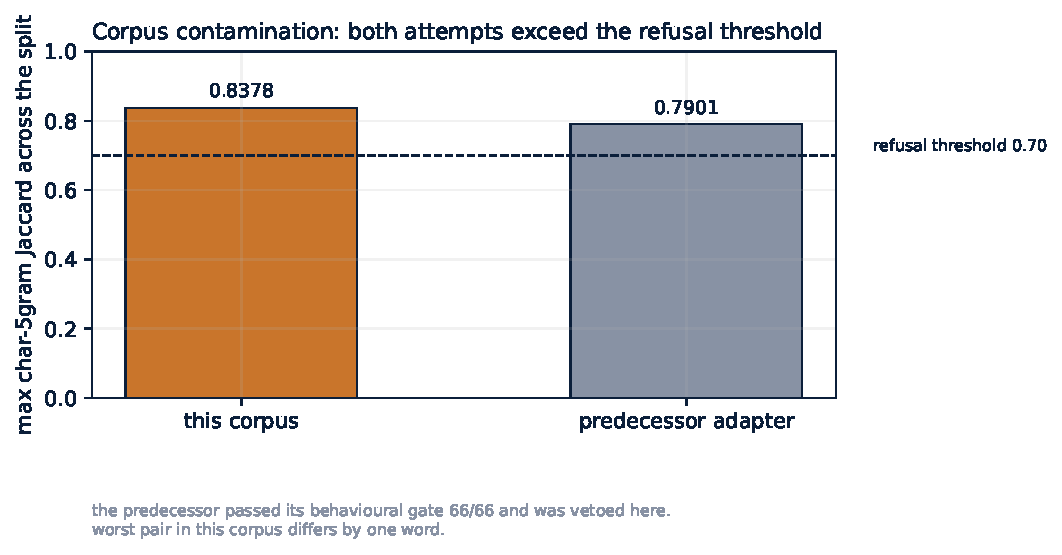
\includegraphics[width=0.74\textwidth]{figures/fig4_leakage.pdf}
\caption{Contamination in two successive attempts at the same task. The predecessor adapter passed its
behavioural gate on every held-out row and was refused on contamination; this work's corpus is
worse.}\label{fig:leak}
\end{figure}

A predecessor adapter distilling this engine reported perfect label and state accuracy, zero malformed
outputs, zero false labels on refusal and zero ungrounded evidence spans, then failed a leakage check at
a mean cross-split cosine of $0.9792$ over $17{,}292$ pairs, with most held-out rows flagged. The rows
were template-generated and split per row rather than per template family, so the held-out set measured
template recall.

We transplanted the refusing form of that check and applied it to this work's corpus, which it refuses.
The worst cross-split pair differs by a single word. We therefore train nothing and publish no weights.

\section{A ledger instead of a narrative}
\begin{figure}[t]\centering
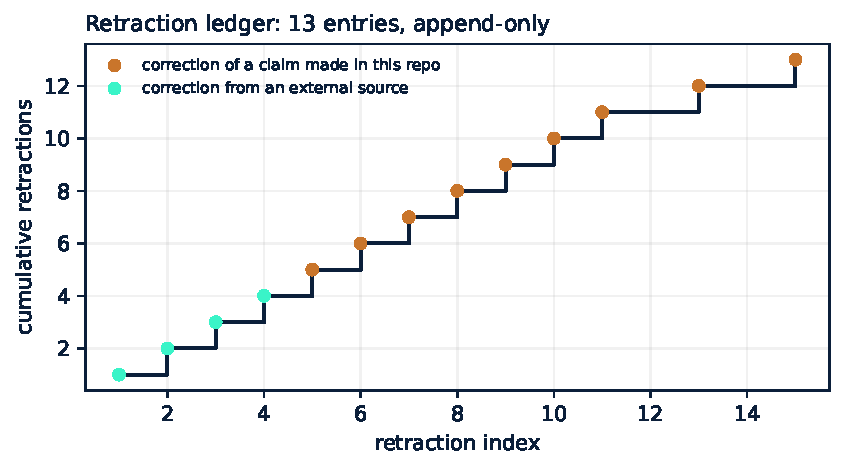
\includegraphics[width=0.74\textwidth]{figures/fig5_retractions.pdf}
\caption{The retraction ledger. Entries are appended, never edited, and each is paired with a test that
prevents the retracted claim from returning.}\label{fig:ret}
\end{figure}

Of 13 retractions, 9 correct claims made earlier in this same work,
including two that were wrong in the direction that flattered it. A checking apparatus that cannot be
disarmed matters more than one that is initially correct: the phrasing guard in this work was silently
neutered by a bulk edit that replaced a forbidden term inside the guard's own pattern list, after which
it matched only its own euphemism. The repair added a test asserting that the guard still names what it
forbids.

\section{Discussion}
None of the three findings required a new method. They required performing comparisons that were already
possible and reporting the result when it was unflattering. The estate had already built every instrument
used here: a Lean formalisation, a labelled gate corpus, a refusing leakage gate, mutation testing for
receipt verifiers, and a benchmark ledger structurally incapable of naming a winner.

We claim this generalises as a practice and not as a capability. A deployed system should be measured
against its own project's formal specification; the failing property should be reported rather than the
report adjusted; and the instruments should be adversarial toward their owner. Where the system fails,
the failing property is the finding.

\section*{What is not claimed}
No trained model, no beaten baseline, no comparison against another system, and no verification by proof
kernel --- formal symbols are bound by name only. The trust aggregator's unconditional uniqueness is
cited as a conjecture, disproved as stated, with a conditional replacement proved axiom-free. Supply
chain posture is level one honest with level two on the roadmap. Release status is BLOCKED.

\section*{Availability}
All figures are generated from machine-readable receipts in the repository; no value in this paper was
typed by hand. Commit b077521.

\end{document}
